\section{选题的背景和意义}

模型检测(Model Checking)是一种自动化形式方法,用于验证有限状态系统的性质。模型检测最初由 E. M. Clarke 和 E. A. Emerson 提出\citep{Emerson_1980,Clarke,Clarke_1986},如今已广泛应用于软件和硬件设计。例如,在嵌入式系统中,可以使用 UML 活动图来验证硬件是否符合规范\citep{Grobelna_2015}。

模型检测将待检测的系统建模为一个跃迁系统(transition system),在时序逻辑(temporal logic)中指定待验证的属性。给定模型\(M\) 和属性\(\varphi\),模型检测将验证是否\(M\)满足\(\varphi\)。在不同的模型检测方法中,高级符号模型检查(Advanced Symbolic Model Checking)\citep{Grobelna_2015}使用简化的有序二叉决策图(Reduced Ordered Binary Decision Diagrams,ROBDDs 或 BDDs)\citep{Bryant_1986}来表示状态集合和转移关系。通过迭代调用图像计算算法来计算所有可达状态,判断一个模型是否满足时间属性,直到达到不动点为止。

最近,随着量子计算的发展,关于量子线路的验证技术也在不断发展\citep{viamontes2007checking,burgholzer2020advanced}。其中,利用模型检测方法对线路进行自动化验证也有了一些应用。由于量子线路运算空间随着量子比特的线性增加而指数级膨胀,传统的计算方法并不能很好应对。因此本次研究希望应用基于张量网络(tensor network)的张量决策图(tensor decision diagrams)进行量子模型检测。 
\subsection{量子计算简介}

量子计算机(quantum computer)是一种利用量子比特特性进行计算的一种设备。在量子计算中,量子比特的特殊性质允许其同时处于多种状态,这与经典比特的二进制状态不同。量子计算机的状态空间可以用希尔伯特空间(Hilbert space)\(\mathcal{H}\)表示\citep{nielsen2010quantum},即可以进行内积运算(inner product)的复向量空间。比特状态可以用\(\mathcal{H}\)的向量表示,量子门由\(\mathcal{H}\)上的酉算子(unitary operator)表示。

量子线路(quantum circuit)是一种描述量子计算的模型。在量子线路中,通过量子比特的初始化、应用量子门、测量以及其他可能的操作的序列来构建和执行量子计算任务。量子线路通常从左向右阅读,每个量子门的作用是将输入的量子比特状态转变为输出状态,该过程可以认为是量子门的酉矩阵与输入的量子状态的乘积。
\begin{figure}[!htbp]
    \centering
    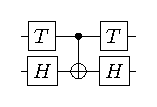
\includegraphics[width=.6\textwidth]{Img/example_cir.pdf}
    \caption{一个量子线路的例子}
    \label{fig:example_cir}
\end{figure}

图\ref{fig:example_cir} 所示的量子线路展示了一个具体的量子线路示例。其中有单比特门\(H=\frac{1}{\sqrt2}\left[\begin{matrix}1&1\\1&-1\\\end{matrix}\right],T=\left[\begin{matrix}1&0\\0&e^{-i\pi/4}\\\end{matrix}\right]\),以及双比特门\(CX=\left[\begin{matrix}\begin{matrix}1&0\\0&1\\\end{matrix}&\begin{matrix}0&0\\0&0\\\end{matrix}\\\begin{matrix}0&0\\0&0\\\end{matrix}&\begin{matrix}0&1\\1&0\\\end{matrix}\\\end{matrix}\right]\)。假设该量子线路的初始状态为\(\left|\psi\right\rangle=\left|\psi_1\right\rangle\left|\psi_2\right\rangle\),则输出状态为\(T\otimes H\cdot CX\cdot T\otimes H\cdot\left|\psi\right\rangle\)。

在量子计算机上可以执行各种算法和计算任务,如量子搜索\citep{Grover_1996}、量子因子分解\citep{shor}和量子模拟\citep{Feynman}等。量子计算的潜力在于其能够在某些特定问题上比经典计算机更高效地进行计算,尤其在处理大规模数据和解决复杂问题方面具有潜在优势。需要对这部分深入了解的读者,可以自行阅读\citep{nielsen2010quantum}。
% //TODO:增加量子计算的重要性
\subsection{量子计算中模型检验的作用与挑战}
%// TODO:加入一些实际例子与具体挑战
\subsubsection{跃迁系统}
跃迁系统广泛应用于模型检测中待检测系统的建模,其定义为\citep{baier2008principles}:
\begin{equation}
\mathcal{M}=\{S,Act,\rightarrow,I\}
\end{equation}
其中\(S\)为系统状态集合,\(I\)为系统初态集合,因此满足\(I\subseteq S\)。\(Act\)为系统行为集合。\(\rightarrow\)为系统状态转移关系,即\(\rightarrow\subset S\times Act\times S\)。此外还有\(AP\)为描述系统原子命题。L是标记函数,将状态映射为状态满足的原子命题集合。需要验证的属性\(\varphi\)将表述为命题。


系统的有限路径片段\(\pi\)是一个有限状态序列\(s_0,s_1\ldots s_n\)。\(s_i\)满足\(s_{i-1}\overset{a}{\rightarrow}s_i,a\in Act\),对于所有\(0<i\leq n\),其中\(n\geq 0 \)。无限路径片段\(\pi\)是一个无限状态序列\(s_0,s_1\ldots\),使得对于所有\(i>0\),\(s_{i-1} \overset{a}{\rightarrow}  s_i,a\in Act\)。在路径中\(\pi\left[i\right]=s_i,\pi\left[i\right)=s_i\ldots\)。所有以\(s_0\)为开始的路径,构成了路径集合\(Path\left(s_0\right)\)。

\begin{figure}[!htbp]
    \centering
    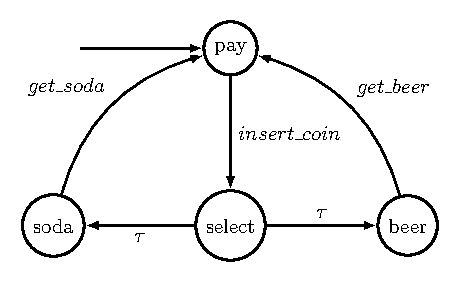
\includegraphics[width=.6\textwidth]{Img/map.pdf}
    \caption{一种简化版的售货机跃迁系统}
    \label{fig:transition-system}
\end{figure}

图\ref{fig:transition-system} 所示的跃迁系统展示了一个简化版的售货机模型。在该模型中,用户投入硬币,进行选择后就可以得到苏打水或者啤酒。在该例子中,系统状态\(S=\{pay,select,soda,beer\}\),系统初态\(I=pay\)。
系统行为\(Act=\{insert\_coin,\tau,get\_soda,get\_beer\}\),其中\(\tau\)表示立即行动符号。转移关系图中已经展示。原子命题可取\(AP=\{paid,drink\}\)。因此\(L\left( pay \right)=\{\varnothing\}\),\(L\left(soda\right)=L\left(beer\right)=\{paid,drink\}\),\(L\left(select\right)=\{paid\}\)。系统的一个路径是\(\pi=pay\ select\ soda\ pay\ selsect\ \ldots\)。此时\(\pi\left[1\right]=slect,\pi\left[1\right)=select\quad soda\quad pay\quad selsect\ldots\)。同时该路径满足\(\pi\in Path\left(pay\right)\)。
量子模型检测的跃迁系统类似。区别在于状态空间用\(\mathcal{H}\),转移关系用酉矩阵。一个量子自动机定义如下:
\begin{align}
    \mathcal{M}=\{\mathcal{H},Act,\{U_\alpha,\alpha\in Act\},\mathcal{H}_0\}
\end{align}
由于目前量子模型检测的发展还比较初期,因此需要验证的属性\(\varphi\)会表示为\(\mathcal{H}\)的一个子空间。
\subsubsection{时序逻辑}
在量子模型检测中,与经典模型检测一样使用时序逻辑指定待验证的属性\(\varphi\)。时序逻辑命题的运算符有两类\citep{goranko_2023}。状态命题公式(State formulas):\(\varphi ::=a\left|\exists\varphi\right|\forall \varphi\left|\lnot\varphi\right|\varphi\land\psi\),其中\(a\in AP\)。以及路径命题公式(Path formulas):\(\varphi\Colon=O\varphi|\varphi U\psi\)。给定模型的一个状态为\(s\),路径为\(\pi\),则具体满足条件分别如下:
\begin{itemize}
    \item \(s\models a,iff \L\left(s\right)\models a\)
    \item \(s\models\exists\varphi,iff\ \pi\models\varphi\)对一些\(\pi\in Path\left(s\right)\)
    \item \(s\models\forall\varphi,iff\ \pi\models\varphi\)对所有\(π\in Paths\)
    \item \(s\models\lnot\varphi,iff\ s\nvDash\varphi\)
    \item \(s\models\varphi\land\psi,iff\ s\models\varphi\ and\ s\models\psi\)
    \item \(\pi\models O\varphi,iff\ \pi\left[1\right]\models\varphi\)
    \item \(\pi\models\varphi U\psi,iff\ \exists j\geq0\).\(\pi\left[j\right)\models\psi\) 同时对所有\(0\le i<j\)有\(\pi\left[i\right)\models\varphi\)
\end{itemize}


图\ref{fig:path-formula-basic} 展示了两种路径命题公式的直观示意图。


\begin{figure}[!htbp]
    \centering
    \begin{subfigure}[b]{0.8\textwidth}
        \centering
        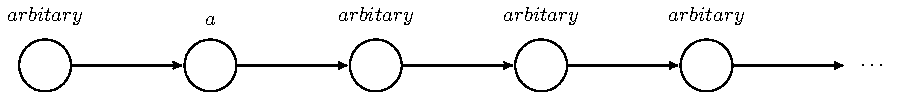
\includegraphics[width=\textwidth]{Img/path_for_Oa.pdf}
    \end{subfigure}
    \\
    \begin{subfigure}{0.8\textwidth}
        \centering
        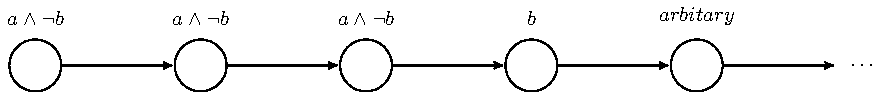
\includegraphics[width=\textwidth]{Img/path_for_aUb.pdf}
    \end{subfigure}
    \caption{$\pi\models O a $与 $\pi\models a U b$的图示}
    \label{fig:path-formula-basic}
\end{figure}
\subsubsection{量子模型检测的应用}
\subsection{当前量子模型检验的问题与研究空间}
\subsubsection{可达性问题}
在模型检测中,有三类比较重要的可达性问题,分别是可达性、持续可达性以及重复可达性。过程中主要涉及以下路径命题公式:\(\lozenge\) 表示最终(eventually),\(\square\)表示总是(always),\(\lozenge\square\)表示总是最终(always eventually),\(\square\lozenge\)表示最终总是(eventually always)。其中\(\lozenge\)和\(\square\)具体定义为:
\begin{itemize}
    \item \(\lozenge\varphi\overset{\text{def} }{=} \text{True}U\varphi\)
    \item \(\square\varphi\overset{\text{def} }{=} \neg\lozenge\neg\varphi\)
\end{itemize}
图\ref{fig:path-formula}展示了这两种基本路径命题公式的直观示意图。
\begin{figure}[!htbp]
    \centering
    \begin{subfigure}[b]{0.8\textwidth}
        \centering
        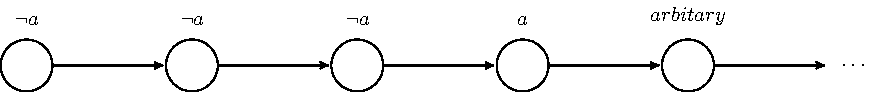
\includegraphics[width=\textwidth]{Img/path_for_Dia.pdf}
    \end{subfigure}
    \\
    \begin{subfigure}{0.8\textwidth}
        \centering
        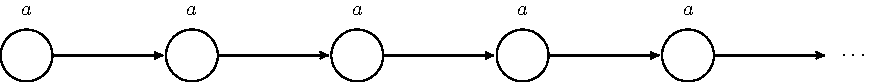
\includegraphics[width=\textwidth]{Img/path_for_SQa.pdf}
    \end{subfigure}
    \caption{$\pi\models\lozenge a$与 $\pi\models\square a$的图示}
    \label{fig:path-formula}
\end{figure}

具体的可满足条件为:
\begin{itemize}
    \item \(\pi\models\lozenge\varphi,iff\exists j\ge0.\pi[j)\models\varphi\)
    \item \(\pi\models\square\varphi,iff\forall j\ge 0.\pi[j)\models\varphi\)
    \item \(\pi\models\lozenge\square\varphi,iff\exists i\ge 0.\forall j\ge i,\pi[j)\models\varphi\)
    \item \(\pi\models\square\lozenge\varphi,iff\forall i\ge 0.\exists j\ge i,\pi[j)\models\varphi\)
\end{itemize}
基于此三种可达性问题定义分别如下:
\begin{itemize}
    \item 可达性:\( Pr^{\mathcal{M}}(s \models \lozenge G) = Pr^M(\pi \models \lozenge G : \pi \in \text{Paths}(s))\)
    \item 持续可达性:\( Pr^{\mathcal{M}}(s \models \lozenge \square G) = Pr^M(\pi \models \lozenge \square G : \pi \in \text{Paths}(s))\)
    \item 重复可达性:\( Pr^{\mathcal{M}}(s \models\square \lozenge G) = Pr^M(\pi \models \square\lozenge G : \pi \in \text{Paths}(s))\)
\end{itemize}
	

\subsubsection{研究空间}
\subsection{研究的潜在应用和影响}
%//TODO:前一节简单介绍
对于量子模型检测的可达性问题的解决,一种直接的解决办法是计算路径上每个状态,然后与待检测属性比较。但是量子计算中状态空间\(\mathcal{H}\)维度\(dim\left(\mathcal{H}\right)=2^n\),其中n为比特数量。即状态空间维数随比特个数指数级增长。因此需要使用新的数据结构,以降低复杂度。

借助更好的数据结构,可以更方便的表示量子状态以及量子线路,并计算最终的结果。比如TDD给出了量子电路的紧凑表示,提供了一种方便的实现张量网络各种操作的方式,这些操作对于模拟量子物理系统非常重要。图\ref{fig:P}展示了一个矩阵和TDD形式,其中TDD中的实线表示高边,虚线表示低边。可以明显看到TDD的结构更紧凑。
 	 
\begin{figure}[!htbp]
    \begin{subfigure}[c]{0.4\textwidth}
        \centering
        \includegraphics[width=\textwidth]{Img/matrix_of_tdd.pdf}
        \caption{矩阵$P$的矩阵形式}
        \label{fig:mat_P}
    \end{subfigure}
    \begin{subfigure}[c]{0.4\textwidth}
        \centering
        \includegraphics[height=6cm]{Img/tdd_ex.pdf}
        \caption{矩阵$P$的TDD形式}
        \label{fig:tdd_P}
    \end{subfigure}
    \caption{应用TDD可以减少存储特殊矩阵的资源}
    \label{fig:P}
\end{figure}

TDD特别适用于实现可达性分析和模型检查算法。这是因为基于BDD的模型检查算法中使用的许多优化技术可以推广到收缩量子电路张量网络上\citep{Chaki_2018}。这些为应用TDD解决量子模型检测问题提供了可能的方案。目前量子模型检测仅仅应用于小
